%!TEX root = Slic3r-Manual.tex

\section{Speed} % (fold)
\label{sec:speed}
\index{speed}
\index{vitesse}

Une fois que l'imprimante produit de manière fiable des impressions de bonne qualité, il peut être souhaitable d'augmenter la vitesse. Faire cela offre plusieurs avantages, le plus évident est que les résultats sont produits plus rapidement, mais aussi que le temps d'impression plus court peuvent être utilisés dans la production de plus de couches, pour la même hauteur de couche, améliorant ainsi la qualité d'impression perçue. Un avantage supplémentaire est qu'un mouvement plus rapide de déplacement entre les extrusions, peut réduire les effets de suintement.

La meilleure approche consiste à incrémenter les différents paramètres de vitesses par petites étapes et observer l'effet de chaque changement a sur la qualité d'impression. La vitesse de déplacement (travel speed) est un point de départ sur, et il n'est pas irréaliste d'atteindre des vitesses allant jusqu'à 250mm/s (si votre imprimante peut le gérer). Les réglages de la vitesse de périmètres (périmeters), de remplissage (infill) sont disponible en mode simple, et la règle générale est que le périmètre aille plus lentement que le remplissage afin de réduire les imperfections éventuelles sur la surface (remplissage peut être plus rapide parce que de légers défauts ne seront que importants).

Le Mode Expert offre plus de paramètres pour régler finement la vitesse de l'imprimante. La différenciation entre les périmètres extérieurs (external), petits (small) et d'autres périmètres, remplissage (infill), et les ponts (bridge)et les vide (gap) sont disponibles, ainsi que la capacité de ralentir la première couche.

\begin{figure}[H]
\centering
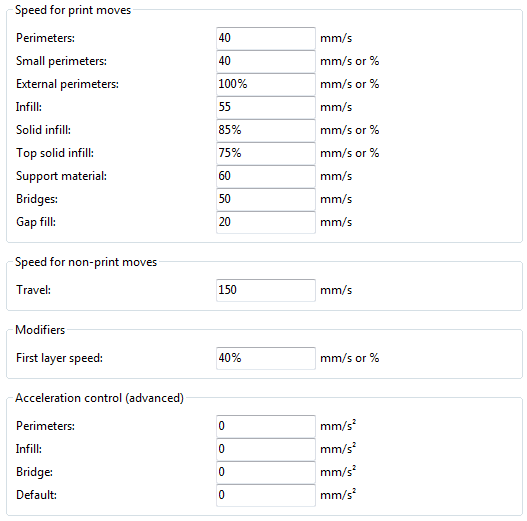
\includegraphics[keepaspectratio=true,width=1\textwidth]{expertmode/speed_advanced_settings.png}
\caption{Paramètres de vitesse en mode expert.}
\label{fig:speed_advanced_settings}
\end{figure}


Le cas échéant, une valeur peut être donnée en pourcentage. C'est par rapport à la valeur précédente, par exemple 50\% de remplissage solide sera la moitié de la valeur définie pour le remplissage.
\index{Print Settings!Speed}
\index{Paramètres d'Impression!Vitesse}
\index{Print Settings!Speed!Perimeters}
\index{Paramètres d'Impression!Vitesse!Périmètres}
\index{Print Settings!Speed!Small perimeters}
\index{Paramètres d'Impression!Vitesse!Périmètres courts}
\index{Print Settings!Speed!External perimeters}
\index{Paramètres d'Impression!Vitesse!Périmètres externes}
\index{Print Settings!Speed!Infill}
\index{Paramètres d'Impression!Vitesse!Remplissage}
\index{Print Settings!Speed!Solid infill}
\index{Paramètres d'Impression!Vitesse!Remplissage plein}
\index{Print Settings!Speed!Top solid }
\index{Paramètres d'Impression!Vitesse!Haut plein}
\index{Print Settings!Speed!Support material}
\index{Paramètres d'Impression!Vitesse!Support}
\index{Print Settings!Speed!Bridges}
\index{Paramètres d'Impression!Vitesse!Pont}
\index{Print Settings!Speed!Gap fill}
\index{Paramètres d'Impression!Vitesse!Remplissage des trous}
\index{Print Settings!Speed!Travel}
\index{Paramètres d'Impression!Vitesse!Déplacement}
\index{Print Settings!Speed!First layer speed}
\index{Paramètres d'Impression!Vitesse!Vitesse de la première couche}

Quelques directives générales pour chaque option:
\begin{itemize}
	\item \texttt{Perimeters} (périmètres) - En mode expert ce paramètre peut être légèrement suppérieur que le paramètre \texttt{External perimeters} (périmètres externes), peut être utilisé pour assurer les faces externes sans défaut.
	\item \texttt{Small perimeters} (petits périmètres) - Conçu pour les trous, les îles et les détails fins, une vitesse plus lente ici est recommandée.
	\item \texttt{External perimeters} (périmètres externes) - Une valeur légèrement plus lente peut assurer des surfaces propres.
	\item \texttt{Infill} (remplissage) - Aussi vite que vous le pouvez sans compromettre l'intégrité de la structure de remplissage. Les extrusions rapides peuvent se briser et entraîner des points faibles.
	\item \texttt{Solid infill} (remplissage solid) - L'extrusion pour le fond du modèle, et les couches solides supplémentaires est généralement un peu plus lente que le pour remplissage mais plus rapide que pour les périmètres.
	\item \texttt{Top solid infill} (remplissage solid du dessus) - Prévoyez du temps pour que l'extrusion couvre proprement les couches supérieures précédentes qu'elle aboutisse à une surface supérieure soigné. les dernières couches doivent parfaitement comblées la structure de remplissage, préparer la voie à une finition soignée.
	\item \texttt{Support material} (support) - Généralement les structures d'appui sont rapide et sale, et tant que que la base est correctement supportée, ils peuvent être construits aussi rapidement que possible.
	\item \texttt{Bridges} (ponts) - Obtenir une distance d'extrusion de portée dépend de la matière et du refroidissement. Aller trop lentement se traduira par l'affaissement, trop rapidement entraînera des brins cassés. L'expérimentation est ici la clé, mais généralement les pontages se réalise plus lentement que les périmètres.
	\item \texttt{Gap fill} (remplissage des vides) - Le remplissage de petits vides engendre de rapide oscillations de l'extrudeuse, la résultante des tremblements et résonance pourrait avoir un effet néfaste sur l'imprimante. Une valeur inférieure peut ici s'en prémunir cela. Un réglage à zéro désactive le remplissage de vide complètement.
	\item \texttt{Travel} (déplacement) - Aussi rapidement que votre imprimante permette afin de minimiser les suintements.
	\item \texttt{First layer speed} (vitesse de la 1ere couche) - Comme mentionné dans la section \ref{sec:the_important_first_layer}, fixer correctement la premère couche est important, et un rythme plus lent aide énormément. Définir un valeur de 50\%, voire moins, peut vraiment aider.
\end{itemize}

\index{Print Settings!Speed!Acceleration control}
\index{Paramètres d'Impression!Vitesse!Crontrole de l'accélération}
\texttt{Acceleration control} est un paramètre avancé permettant les paramètres d'accélération pour les périmètres, remplissage, pont, ainsi que d'un réglage par défaut, à faire. Décider quelles valeurs régler dépend des capacités de la machine. Tous les paramètres dans le firmware peuvent être un bon point de départ.

Tenir compte des restrictions imposées par le firmware comme beaucoup ont des paramètres de vitesse de sécurité maximale pour chaque axe.

% section speed (end)